\subsection{Experiment}
To verify our method using physical hardware, we developed an AVR application which continuously generate an increasing integer sequence and send the it to the UART interface at a controllable speed. An Python program running on a desktop is used to observe the impact of the bit flips by monitoring the interger sequence. T interrupt function is used to generate a random address within the range from the top of the stack to the  at random location of the used RAM space of the AVR microprocessor. A Python program running on a desktop is used to receive the integer sequence on a PC and to observe the correctness of the running status of the AVR application.

\begin{table*}
	\center
    \begin{tabular}{|l|c|c|c|c|}
    \hline
   \textbf{Timer Prescaler}   & \textbf{Interval = 1ms} & \textbf{Interval = 10ms} & \textbf{Interval = 100ms} & \textbf{Interval = 1000ms}	\\ \hline
    1      	& 27			& 1				& 0				& 0				\\ \hline
    8       & 149			& 48			& 46           	& 0				\\ \hline
    64      & 1000			& 838			& 259		   	& 8				\\ \hline
    256		& 3333			& 2478			& 460      		& 120			\\ \hline
    1024    & 10331			& 4103			& 848           & 1164			\\ \hline
    \end{tabular}
	\vspace{5pt}
    \caption {Maximum Number Sent Out}
    \label{tbl_exp1_result}
\end{table*}
In the experiment, the microprocessor runs at $10^7$Hz. The prescaler for the timer to trigger the interrupt have been set to 1, 8, 64, 256, and 1024. With different interrupt trigger interval, the frequency of the error insertion can be calculated. In the meanwhile, \textit{delay} is also used to control the speed of the number sending. The results of maximum number sent out in terms of error insertion frequency and number sending interval(\textit{ms}) are summerized in Figure \ref{fig:exp1_result}. The x-axis represents the error insertion frequency, the y-axis represents the maximum number the Python program received on PC. The figure shows that given the same speed of number sending, the higher the error insertion frequency is, the less numbers will be sent out; while given the same error insertion frequency, the higher speed the program is running, the more numbers will be sent out. This result reveals that the higher error insertion frequency is, the higher probability the SEUs will occur on critical area, which makes the program crashes. The program execution speed also have impact on the consequence of the SEUs. However, as the error insertion frequency increases, the difference of the time before the program crash decreases dramatically. When the error insertion frequency is extremely high, the program can hardly send anything.

\begin{figure}
\centering
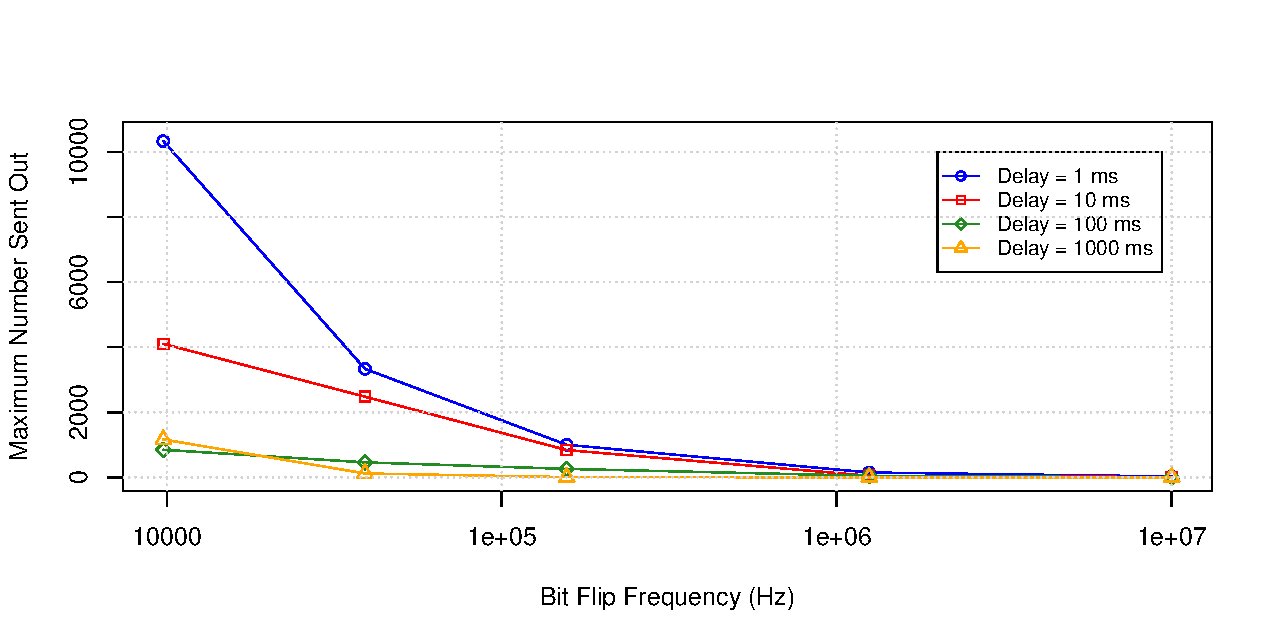
\includegraphics[scale=0.4]{figures/experiment1.pdf}
\caption{Error Insertion}
\vspace{5pt}
\label{fig:exp1_result}
\end{figure}

